\chapter{Conceptos básicos}
\label{chap:conceptos_basicos}

\lettrine{P}{ara} una correcta comprensión de los objetivos de este trabajo, tanto a corto como a largo plazo, es necesario conocer una serie de conceptos básicos relacionados con las redes neuronales, su estructura, rendimiento y cómo se implementan en un procesador moderno, para posteriormente poder comprender las mejoras propuestas a continuación.

\section{Redes neuronales}
\label{sec:redes_neuronales}
Las redes neuronales constituyen la base de la mayoría de los últimos avances en el campo de la inteligencia artificial. A pesar de la enorme diversidad en \textit{layouts} de capas, neuronas, funciones de transferencia, etc., la realidad es que el álgebra lineal y la multiplicación de matrices son parte fundamental e imprescindible para la ejecución de las mismas \cite[Figura 3.4]{deep_learning_for_computer_architects}.

A pesar de que en la Prueba de Concepto (\acrlong{poc} o \acrshort{poc} por sus siglas en inglés) expuesta en el Capítulo \ref{chap:desarrollo_poc} se trabaja únicamente con redes \textit{feed-forward}, sería naíf pensar que solamente existen estas arquitecturas de redes neuronales. Ejemplos a destacar pueden ser las redes convolucionales, empleadas principalmente para el procesado de imágenes, las basadas en modelos secuenciales o en \textit{transformers}, que están revolucionando el mundo de la inteligencia artificial mediante modelos de procesamiento del lenguaje o de generación de imágenes, así como muchas otras como las redes GAN, o las basadas en arquitecturas \textit{encoder-decoder}.

Estas arquitecturas son llamadas de redes neuronales, a pesar de que, como es evidente, una neurona no puede como tal ``ejecutar'' una convolución. Más bien, estas nuevas arquitecturas se basan en la modelación de operaciones matemáticas complejas en pasos discretos, como por ejemplo la convolución anteriormente mencionada.

\subsection{Estructura de una red neuronal \textit{feed-forward}}
\label{ssec:estructura_red_neuronal_ff}
Las redes neuronales \textit{feed-forward} se componen de varias capas de neuronas que toman una o más entradas, realizan la suma de todas ellas, suman un \textit{bias}, y finalmente aplican una función de transferencia no lineal.

La capa que toma los datos de entrada se llama capa \textit{input} o de entrada, y la capa que expulsa los datos de salida es la capa \textit{output} o de salida. Las capas que realizan transformaciones intermedias se denominan capas ocultas o \textit{hidden layers}.

En la Figura \ref{fig:dense_nn_sample}\footnote{Imagen generada con la herramienta NN-SVG, disponible en \url{https://alexlenail.me/NN-SVG}} se puede ver un diagrama de una red neuronal \textit{feed-forward} densa. Esto es, una red neuronal en la que cada neurona de una capa está conectada con todas las neuronas de la capa siguiente. Esto se traduce en que la matriz de pesos que representa cada capa es una matriz densa, o dicho de otra manera, que no contiene pesos con valor cero.

\begin{figure}[h!]
    \centering
    \vspace*{0.5cm}
    \def\svgwidth{0.85\textwidth}
    \input{pdf_tex/dense_nn/dense_nn_svgnn.pdf_tex}
    \caption{Red neuronal densa \textit{feed-forward}}
    \label{fig:dense_nn_sample}
\end{figure}

Por el contrario, como se puede ver en la Figura \ref{fig:sparse_nn_sample}, existen las redes neuronales dispersas, en las que una cantidad significativa de los pesos tienen valor cero. Estas redes se pueden obtener de múltiples formas, y sus objetivos son variados, a pesar de que el principal objetivo es reducir el tamaño del modelo.

Uno de los posibles métodos para la obtención de una red neuronal dispersa (\textit{sparse}) es mediante el podado o \textit{pruning}. Este método, sorprendentemente similar al empleado por neurocirujanos durante operaciones a cerebro abierto, consiste en ir cortando conexiones de forma más o menos arbitraria (en función del algoritmo) y observando cómo varía la salida. En caso de que la salida sea correcta, se continúa en esa dirección. Para que un cambio en una red neuronal se considere inapreciable, la salida debe verse alterada de tal forma que sea indistinguible su efecto del de unos diferentes parámetros iniciales durante el entrenamiento. Esto implica que este ``ruido'' será corregible mediante un reentrenamiento y se mide con la métrica \textit{\acrlong{itn}} o \acrshort{itn} \cite[4.1.1]{deep_learning_for_computer_architects}.

De esta forma, una red neuronal dispersa puede contener alrededor de un 80-90\% menos de conexiones entre neuronas, representando esto un ahorro sustancial de energía en términos de acceso a memoria, relevante en sistemas miniaturizados donde cada milivatio cuenta.

\begin{figure}[h!]
    \centering
    \vspace*{0.5cm}
    \def\svgwidth{0.85\textwidth}
    \input{pdf_tex/sparse_nn/sparse_nn_svgnn.pdf_tex}
    \caption{Red neuronal dispersa \textit{feed-forward}}
    \label{fig:sparse_nn_sample}
\end{figure}

Esta operación de podado puede no solamente limitarse a los pesos que interconectan neuronas, sino que se puede hacer el modelo más eficiente y reducido al podar todos los pesos entrantes en una neurona, eliminando por completo dicha neurona, y por tanto eliminando también todas sus conexiones posteriores en cadena. El efecto de eliminar una neurona sin conexiones entrantes, que únicamente arroja valores constantes en cada iteración, se puede compensar ajustando el \textit{bias} del receptor que correspondía a esa neurona en las conexiones posteriores.

\subsection{Redes neuronales profundas}
\label{ssec:redes_reuronales_profundas}
El \textit{boom} de la inteligencia artificial en los últimos años viene dado en gran medida por el enorme crecimiento que ha experimentado el campo mediante técnicas de \textit{deep learning}, precisamente en estas redes neuronales profundas o \textit{deep neural networks}.

Y es que dentro de las infinitas posibilidades que nos ofrecen las neuronas artificiales tratadas anteriormente, existe la posibilidad de apilar capa sobre capa, obteniendo con cada capa extra comportamientos y patrones más complejos.
Es precisamente este comportamiento de los sistemas no lineales el que permite reproducir comportamientos exóticos al aumentar el número de neuronas y/o capas (y por tanto la complejidad) del sistema.

Tras sospechas previas de algunos investigadores como George Cybenko acerca de que una red neuronal con al menos una capa oculta es un aproximador universal, y tras demostrar dicho comportamiento para la sigmoide como función de transferencia \cite{cybenko1989approximation}, Kurt Hornik demostró en 1991 que una red neuronal de con al menos una capa oculta es siempre un aproximador universal, independientemente de la función de transferencia, siempre que esta sea no polinomial. A pesar de que una red neuronal de una sola capa oculta pueda ser un aproximador universal, se obtienen aproximaciones mucho más inteligentes y ``económicas'' computacionalmente al contar con más de una capa oculta \cite{hornik1991approximation}, donde el máximo exponente de esta doctrina es precisamente el \textit{deep learning}.

\section{Redes neuronales densas}
\label{sec:redes_reuronales_densas}
Como se comentó en la sección anterior, independientemente del número de capas de la red, sea profunda o ``convencional'', una red neuronal densa es aquella en la que para $m$ neuronas en la capa $M$, y $n$ neuronas en la capa $N$, donde la neurona $x$ de la capa $M$ se denota $M_{x}$, existe siempre una conexión de $M_{m}$ a $N_{n}$, es decir ($m\longrightarrow n$):

\begin{equation}
\forall m \in M \:\wedge\: \forall n \in N, \: m\longrightarrow n\nonumber
\label{eq:dense_nn}
\end{equation}

De esta forma, para la ejecución (inferencia) de una red neuronal densa \textit{feed-forward}, serán necesarias únicamente una simple multiplicación de matrices, una suma de matrices para tener en cuenta los \textit{bias}, y la aplicación de una función de transferencia.

Esto se puede apreciar en la Figura \ref{fig:nn_matrix_dense}\footnote{Imágenes con este estilo se han obtenido y modificado de \url{https://ml-cheatsheet.readthedocs.io/en/latest/forwardpropagation.html}}. En ella se puede ver el proceso de inferencia de 4 datos bidimensionales, correspondientes con el número de filas de entrada a las capas. Como también se puede apreciar, la anchura de cada capa se corresponde con el número de columnas de la misma.

\begin{figure}[h!]
    \centering
    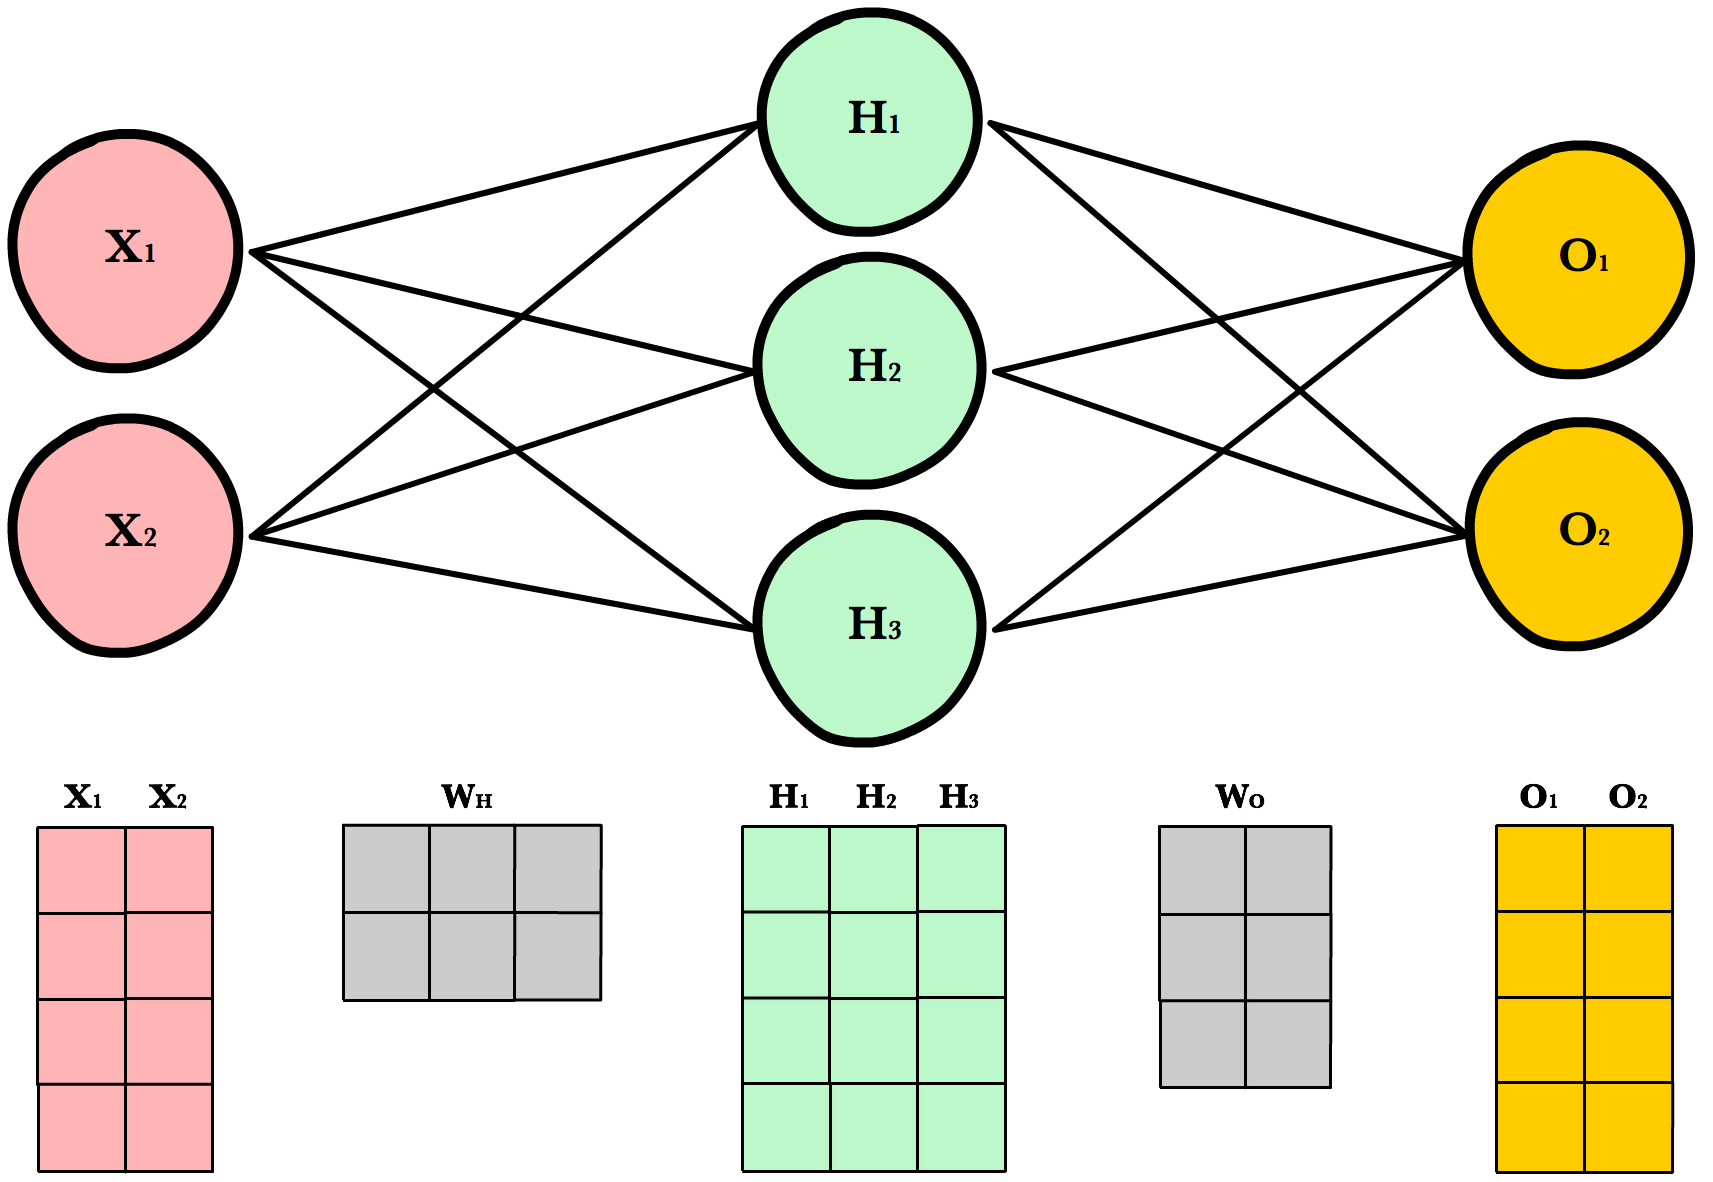
\includegraphics[width=0.85\textwidth]{img/neural_network_matrix_dense.png}
    \caption{Visualización de inferencia en redes neuronales densas}
    \label{fig:nn_matrix_dense}
\end{figure}

Así, si el dato (vectorial por la naturaleza de estas redes) tiene 24 elementos, será necesaria una capa de entrada de 24 neuronas (24 columnas $x_{1} .. x_{24}$ según notación de la Figura \ref{fig:nn_matrix_dense}), y si queremos inferir sobre 1000 de estos datos, esto se puede hacer en una sola ejecución, siendo el número de columnas también de 1000.

O dicho de otra manera, sea la capa $M_{m}$ una capa completamente conexa con $m$ neuronas, a la cual se le introduce un dato $x_{m}$, donde el peso de la neurona $M_{i}$ hacia $N_{j}$ se denota como $w_{M,i,j}$, y la función de transferencia es $\phi$, entonces se tiene que la salida de una capa será:

\begin{equation}
    x_{N,i} = \phi\left(\sum_{j}w_{N,i,j}x_{M,j}\right)\nonumber
    \label{eq:dense_nn_eq}
\end{equation}

A esta función se le puede añadir el \textit{bias} de forma explícita ($\sum\left([\dots] x_{M,j}\right) + bias_{N,i}$), o de forma implícita, siendo el \textit{bias} una conexión más, con un valor constante de 1, cuyo peso es el multiplicador que da el \textit{bias} resultante.

\section{Redes neuronales dispersas}
\label{sec:redes_reuronales_dispersas}
Las redes neuronales dispersas cuentan con una ventaja, y es el menor número de conexiones entre neuronas, o directamente el menor número de neuronas en la arquitectura. A pesar de esto, en realidad el fundamento matemático es el mismo, una simple multiplicación de matrices. Sin embargo, y aunque tengan el mismo funcionamiento base que su contraparte densa, se pueden explotar ciertas características, tanto de la estructura de las matrices dispersas como de su multiplicación, para obtener mejoras tanto en el tamaño del modelo como en su rendimiento, respectivamente.

\subsection{Fundamentos de matrices dispersas}
\label{ssec:fundamentos_matrices_dispersas}
Una matriz es dispersa cuando gran parte de su contenido son únicamente ceros. El cuan dispersa es una matriz se cuantifica mediante el ``grado de dispersión'' o \textit{sparsity}. Una matriz dispersa $10 \times 10$ con tres elementos diferentes de cero (denominados elementos \textit{nonzero} o directamente \textit{nonzeros}) será una matriz dispersa con una \textit{sparsity} del $97\%$ y una densidad del $3\% \:(=100\%-97\%)$.

\subsection{Almacenamiento de matrices dispersas}
\label{ssec:almacenamiento_matrices_dispersas}
Existen múltiples métodos para el almacenamiento de matrices dispersas en memoria, pero uno de los más sencillos de comprender, y que se usa en la \acrshort{poc} para la creación de las matrices dispersas, es el formato \acrshort{coo} o \textit{\acrlong{coo}}.

Este formato consiste en el almacenamiento de dato y coordenadas en tres vectores: \texttt{V}, \texttt{C} y \texttt{R} (\textit{Value}, \textit{Column}, \textit{Row}). Para cada entrada en el vector \texttt{V}, se crea una entrada en la misma posición para los vectores \texttt{C} y \texttt{R}, indicando la columna y fila en la que se ubica el valor \textit{nonzero}. Por diseño, el tamaño de cada uno de estos tres vectores tiene que ser igual al número de \textit{nonzeros}, denotado por \texttt{NZ}. Este formato es particularmente cómodo para la creación de matrices dispersas de forma ágil, pero existen formatos más avanzados, tanto en tamaño como en eficiencia, como el \acrshort{csr} o \textit{\acrlong{csr}}\footnote{Más información en \url{https://en.wikipedia.org/wiki/Sparse_matrix\#Compressed_sparse_row_(CSR,\_CRS\_or\_Yale\_format)}}.

A continuación se muestra un ejemplo de una matriz dispersa almacenada en formato \acrshort{coo}. A pesar de que esta matriz no es particularmente dispersa, se utiliza únicamente con fines explicativos:

\begin{center}
    $\begin{pmatrix}
        1 & 0 & 0 & 0\\
        0 & 2 & 0 & 0\\
        0 & 3 & 4 & 0\\
        0 & 0 & 0 & 5
    \end{pmatrix}$
    \vspace*{0.5cm}
\begin{lstlisting}[]
NZ = 5

V = [ 1 2 3 4 5 ]
C = [ 0 1 1 2 3 ]
R = [ 0 1 2 2 3 ]
\end{lstlisting}
\end{center}

\subsection{Propiedades del producto de matrices dispersas}
\label{ssec:propiedades_producto_matrices_dispersas}
Al multiplicar dos matrices densas no hay duda de que como resultado se obtendrá una matriz densa, salvo contadas excepciones, como multiplicar una matriz por su inversa. Sabiendo que el producto de matrices dispersas obtiene el mismo resultado que una multiplicación de matrices densas mediante un algoritmo diferente, se pueden clasificar los productos de matrices en función de su \textit{sparsity} de forma genérica.

Esta clasificación, de nuevo, puede variar en función de las propiedades de la matriz, pero es la base sobre la cual se construyen las funciones de \acrshort{blas} (\textit{\acrlong{blas}}) \cite{netlib_blas} y las implementaciones Sparse \acrshort{blas} \cite{sparse_blas_10.1145/567806.567810}. De esta forma, se pueden implementar los siguientes tipos de producto de matrices:

\begin{itemize}
    \item Densa $\times$ Densa $=$ Densa ($D\times D$)
    \item Dispersa $\times$ Densa $=$ Densa ($d\times D$)
    \item Dispersa $\times$ Dispersa $=$ Dispersa / Densa\footnote{En función de la forma en que los valores \textit{nonzero} estén dispuestos en ambas matrices, el resultado puede ser una matriz dispersa o densa.} ($d\times d$)
\end{itemize}

Estos tres tipos principales de productos, en típico \textit{BLAS-fashion} se pueden realizar para tipos de datos según su precisión, \texttt{S}, \texttt{D}, \texttt{C} y \texttt{Z} (\textit{Single}, \textit{Double}, \textit{Single Complex}, \textit{Double Complex}).
Así, se pueden obtener las siguientes funciones estándar, a pesar de que en la parte \textit{sparse} de \acrshort{blas} hay menor consenso debido a la existencia de múltiples librerías que difieren del estándar por ser previas a la creación del mismo. Por ejemplo, los tipos especificados en la función se van perdiendo conforme se avanza hacia implementaciones genéricas en C++.

\begin{itemize}
    \item \texttt{[sdcz]gemm()} para $D\times D$
    \item \texttt{[sdcz]usmm()} o \texttt{spmm()} para $d\times D$
    \item \texttt{sp[sdcz]gemm()} o \texttt{spmsp()} para $d\times d$
\end{itemize}

Sabiendo las características de una red neuronal dispersa, y tal como se comenta más adelante en esta memoria, en la \acrshort{poc} se emplea el producto $d\times D$, debido a la naturaleza dispersa de los pesos, y densa de los datos de entrada. De todas formas, en función de la naturaleza de los datos de entrada, podrían emplearse también vectores de entrada dispersos, aunque lo más probable es que para eso quizás una red neuronal \textit{feed-forward} unidimensional no sea lo más apropiado, y ya se deban sugerir otras arquitecturas de red. Redes como las convolucionales, en las que se opera total o parcialmente con matrices que pueden ser dispersas, parecen una mejor idea.

\subsection{Visualización de una red neuronal dispersa}
\label{ssec:visualizacion_nn_dispersa}
Tal como se mostró en la Sección \ref{sec:redes_reuronales_densas}, es sencillo visualizar el proceso de inferencia como una simple multiplicación de matrices, por lo que una multiplicación con una matriz de pesos dispersa debería ser sencilla de visualizar de forma similar.

Este razonamiento es correcto, y es muy sencilla de visualizar de no ser por un pequeño detalle. La función de multiplicación de matrices $d\times D$, \texttt{[sdcz]usmm()}, tiene una firma poco genérica, lo que hace que tenga un sutil detalle que requiere un poco de detenimiento. Si bien la función \texttt{BLAS\_susmm} parece adecuada para esta carga de trabajo, se puede apreciar este pequeño inconveniente en la firma de la función a continuación:

\begin{lstlisting}[language=C]
int BLAS_susmm( enum blas_order_type    order,
                enum blas_trans_type    transA,
                int                     nrhs,
                float                   alpha,
                blas_sparse_matrix      A,
                const float *           b,
                int                     ldb,
                float *                 c,
                int                     ldc 
)

/**
 * order    Layout of the dense array.
 * transA   Transposition operator for matrix A.
 * nrhs     Number of right hand side columns.
 * A        A valid matrix handle.
 * alpha    Value for alpha.
 * b        Dense vector b.
 * ldb      Leading dimension of b.
 * c        Dense vector c.
 * ldc      Leading dimension of c.
 */
\end{lstlisting}

El problema de \texttt{BLAS\_susmm}, que calcula $C = \alpha AB + C$ en simple precisión, es que la matriz $A$ debe ser dispersa, algo que, fijándose de nuevo en la Figura \ref{fig:nn_matrix_dense}, no se cumple. Es decir, la matriz dispersa es la de pesos $w$, por lo que parece necesaria una función que trate a $B$ como una matriz dispersa. Dicha función no existe.

\begin{figure}[h!]
    \centering
    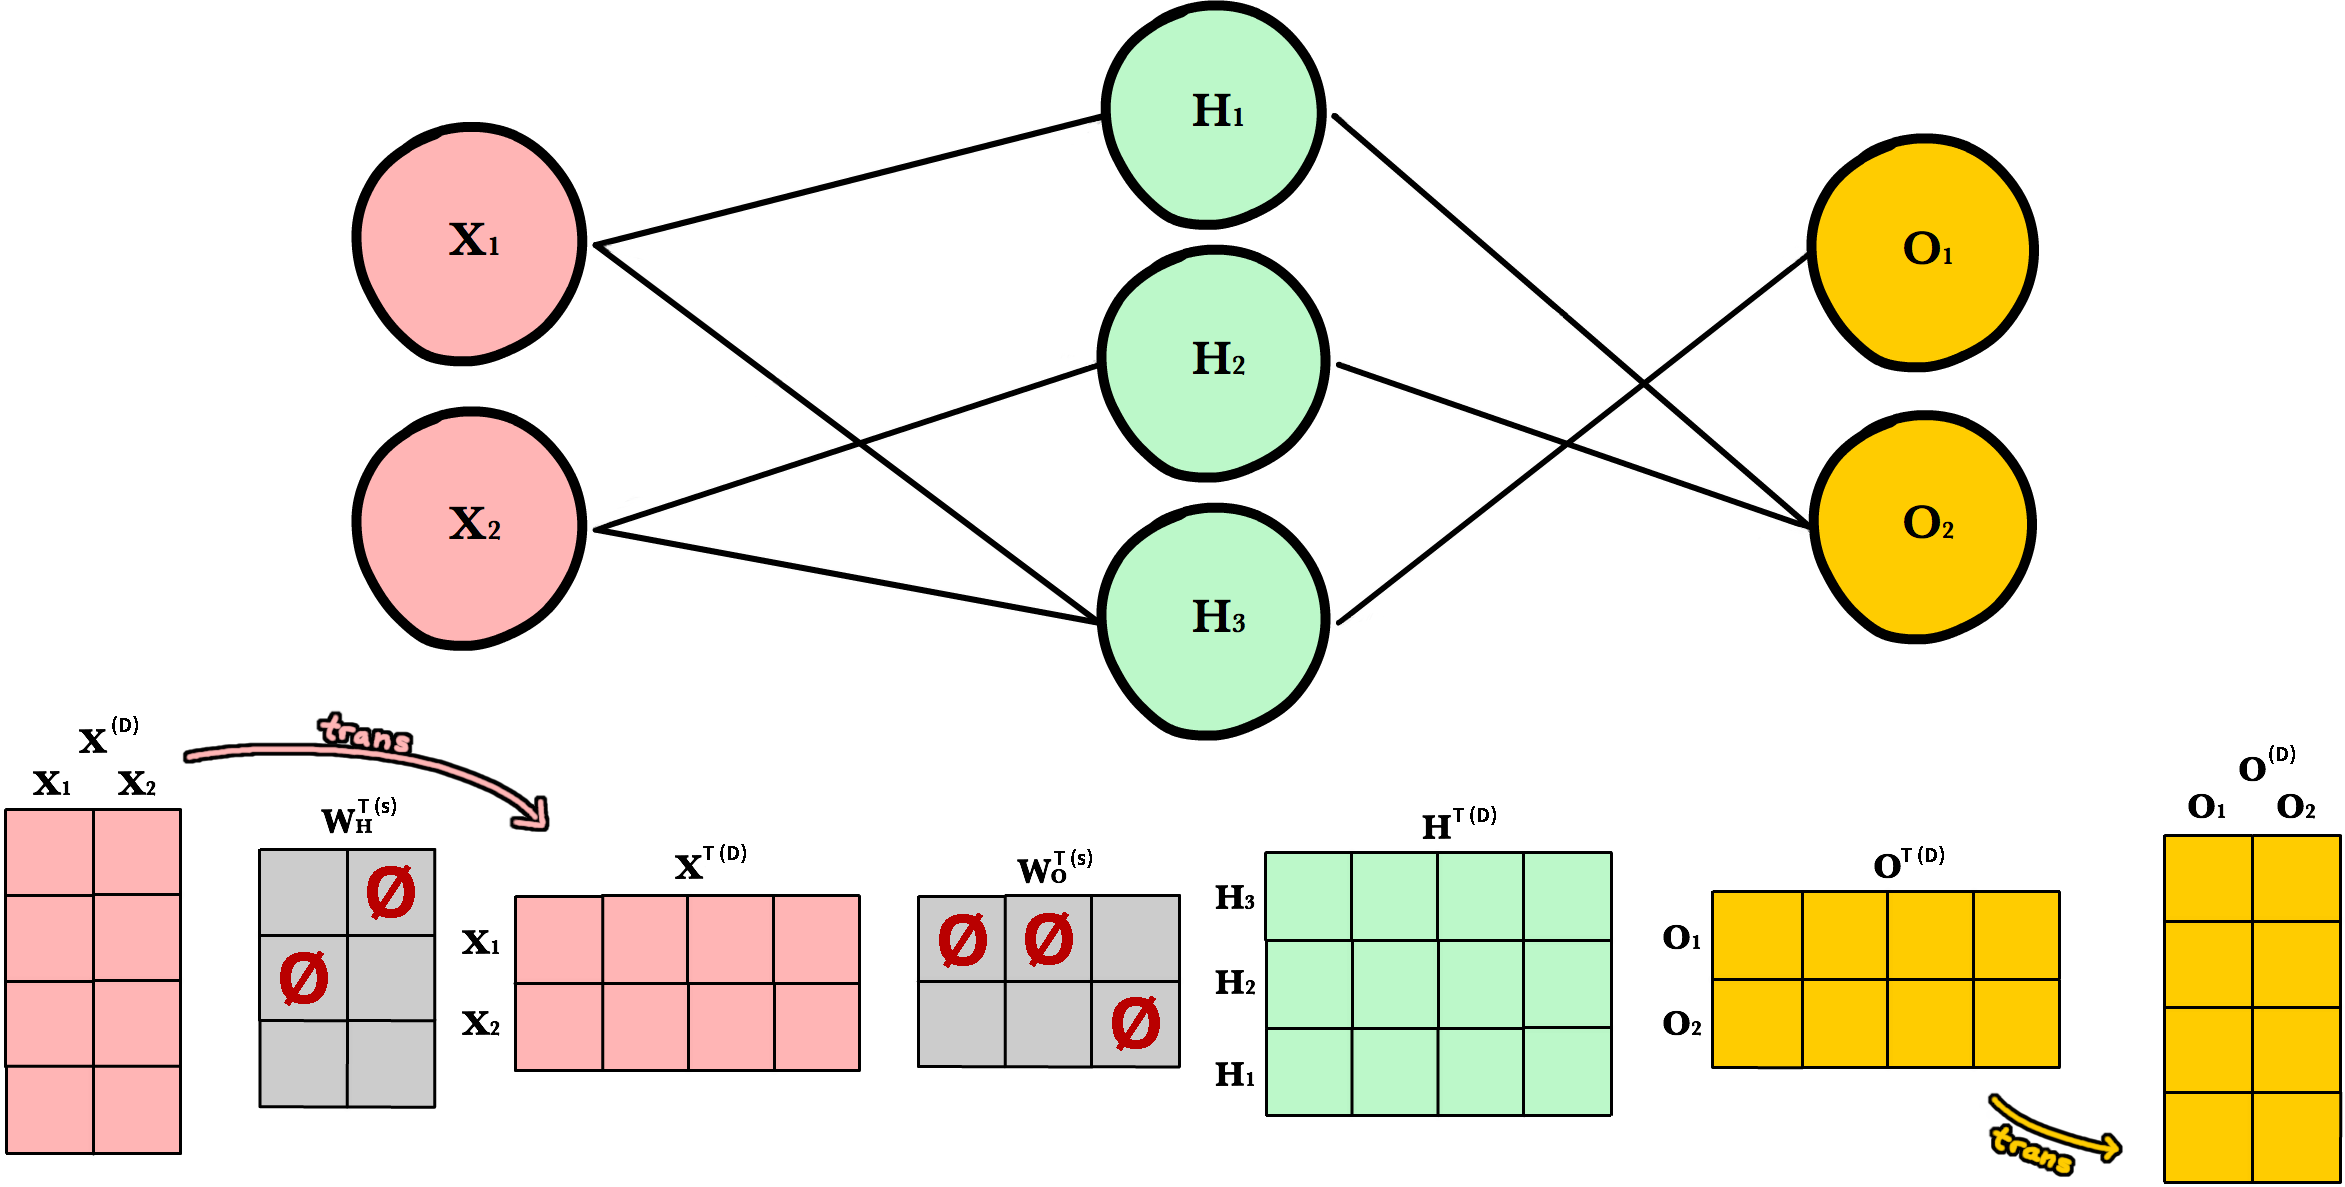
\includegraphics[width=\textwidth]{img/neural_network_matrix_sparse/neural_network_matrix_sparse.png}
    \caption{Visualización de inferencia en redes neuronales dispersas}
    \label{fig:nn_matrix_sparse}
\end{figure}

Sin embargo, empleando las propiedades de las matrices, es posible modificar el orden de las mismas, y así poder encajar cada matriz en la firma. Para esto se emplea una propiedad básica de las matrices, $C^{T} = (AB)^{T} = A^{T}B^{T}$. De esta forma, al transponer la matriz de pesos mediante el parámetro \texttt{transA}, y multiplicando esto por la salida de la capa anterior, se obtiene la salida $C^{T}$. Esto supone un pequeño \textit{overhead}, al tener que transponer la entrada a la capa de entrada, así como la salida de la capa de salida. Sin embargo, dicho \textit{overhead} puede mitigarse en gran medida, en función de la arquitectura de la red, así como de la fuente de datos, que es más que probable que mediante pequeñas modificaciones como filtrado o manejo de ficheros pueda exportar los datos transpuestos de base.

Esta estrategia se puede apreciar en la Figura \ref{fig:nn_matrix_sparse}, donde a diferencia de la Figura \ref{fig:nn_matrix_dense} se han transpuesto los pesos y las entradas, y han sido etiquetados correspondientemente mediante superíndices.

\section{Multiplicación de matrices \textit{point-to-point}}
\label{sec:multiplicacion_point_to_point}
A pesar de todo lo comentado previamente, el empleo de las funciones que ofrecen Sparse \acrshort{blas}, Intel MKL\footnote{\url{https://www.intel.com/content/www/us/en/develop/documentation/get-started-with-mkl-for-dpcpp/top.htmlde ver}} y alternativas, no es la única opción para realizar la multiplicación de matrices dispersas. Una buena aproximación es el empleo de una arquitectura \textit{point-to-point}, que también se podría denominar como \textit{fully unrolled} o \textit{data-specific}. Esta arquitectura consiste en \textit{hardcodear} cada una de las operaciones que intervienen en la multiplicación de matrices dispersas con una línea de \texttt{\acrshort{fma}} (\textit{\acrlong{fma}}) por cada valor \textit{nonzero} (\textit{point}) de la matriz.

Para generar dicho código se necesita tener primero una base teórica. Considérese el siguiente ejemplo: sean dos matrices $d \times D$, de dimensiones $m \times n$ y $n \times k$, respectivamente, teniendo la matriz dispersa una densidad del 50\%, y siendo $\#nz$ el número de valores \textit{nonzero} en la misma:
\begin{gather}
    \begin{pmatrix}
        0 & d_{12}\\
        d_{21} & 0\\
        0 & d_{32}
    \end{pmatrix}	
    \begin{pmatrix}
        D_{11} & \dots\\
        D_{21} & \dots
    \end{pmatrix}
    =
    \begin{pmatrix}
        C_{11} & \dots\\
        C_{21} & \dots\\
        C_{31} & \dots
    \end{pmatrix} \nonumber % https://latex.org/forum/viewtopic.php?t=20368
\end{gather}

Comenzando con la matriz resultado $C$ en una región de memoria a cero, la secuencia de operaciones a realizar sería la siguiente para este ejemplo:
\begin{center}
    $C_{11} \pluseq d_{12} \cdot D_{21}$\\
    $C_{21} \pluseq d_{21} \cdot D_{11}$\\
    $C_{31} \pluseq d_{32} \cdot D_{21}$\\
\end{center}

Esta secuencia \textit{hardcodeada} se repetirá $k$ veces (el número de columnas de $D$ y $C$). Teniendo en cuenta que una operación \texttt{\acrshort{fma}} realiza dos FLOPs, se puede concluir que el número de FLOPs necesarios para el cálculo de la matriz resultado $C$ será $2 \cdot \#nz \cdot k$.

\subsection{Teoría y ventajas de la localidad}
\label{ssec:teoria_ventajas_localidad}
Teniendo en cuenta que, para la matriz de pesos dispersa, sus valores \textit{nonzero} pueden almacenarse en memoria de forma secuencial, y dada la propiedad asociativa de la suma, se puede conseguir un algoritmo de multiplicación de matrices que únicamente realice accesos por filas. Al fin y al cabo todo se reduce a cómo se representan las matrices en memoria.

Por tanto, para una multiplicación de matrices similar a la tratada en esta sección ($w^{d} \times x^{D} = out^{D}$, de dimensiones $m \times n$, $n \times k$ y $m \times k$, respectivamente), se puede representar la dimensión común de medida $n$ en el eje horizontal. La siguiente multiplicación de matrices no está en una disposición compatible, pero tal como se puede apreciar en la siguiente subsección, tenerlas en este \textit{layout} en memoria es muy beneficioso para la localidad de los datos: 
\begin{gather}
    \begin{pmatrix}
        w_{00} & w_{01}\\
        0 & w_{11}\\
        0 & 0\\
        w_{30} & w_{31}
    \end{pmatrix}	
    \begin{pmatrix}
        x_{00} & x_{01}\\
        x_{10} & x_{11}\\
        \vdots & \vdots
    \end{pmatrix}
    =
    \begin{pmatrix}
        out_{00} & out_{01} & out_{02} & out_{03}\\
        out_{10} & out_{11} & out_{12} & out_{13}\\
        \vdots & \vdots & \vdots & \vdots
    \end{pmatrix} \nonumber
\end{gather}

\subsection{Obtención de la secuencia de operaciones}
\label{ssec:obtencion_secuencia_operaciones}
El procedimiento a seguir será multiplicar cada una de las filas de la matriz $w^{d}$ por cada fila de la matriz $x^{D}$, ambas mostradas en la subsección anterior. A cada iteración de la matriz $w^{d}$ se desplazará una posición a la derecha en la matriz $out^{D}$. Sin embargo, primero es conveniente almacenar los valores dispersos de la matriz $w^{d}$. Para esto, se puede construir una \acrshort{lut} (\textit{\acrlong{lut}}). En esta tabla se almacenan cada uno de los valores \textit{nonzero} de la matriz $w^{d}$ recorrida en orden secuencial estilo C. Para este ejemplo, el contenido de la \acrshort{lut} se muestra en la Tabla \ref{tab:lut_example}. En la columna izquierda puede verse la coordenada original del valor ubicado en la posición a su derecha.

\begin{table}[h!]
    \centering
    \begin{tabular}{|c|c|}
    \hline
    \textbf{(x$^{\sharp}$,y$^{\flat}$)} & \textbf{pos$^{\natural}$} \\\hline
    (0,0) & 0 \\\hline
    (0,1) & 1 \\\hline
    (1,1) & 2 \\\hline
    (3,0) & 3 \\\hline
    (3,1) & 4 \\\hline
    \end{tabular}
    \caption{Contenido de la LUT para la matriz $w^{d}$. \textbf{x}, \textbf{y} y \textbf{pos} se etiquetan con $\sharp$, {\large$\flat$} y $\natural$}
    \label{tab:lut_example}
\end{table}

A su vez, en la Tabla \ref{tab:w_matrix_memory_layout} se puede ver la disposición en memoria de cada valor \textit{nonzero} de la matriz dispersa de pesos que, debido a la omisión de los ceros en $w^{d}$ se almacenan forma contigua en memoria.

\begin{table}[h!]
    \centering
    \begin{tabular}{|c|c|c|c|c|c|}
        \hline
        \textbf{pos} & 0 & 1 & 2 & 3 & 4 \\\hline
        \textbf{val} & $w_{00}$ & $w_{01}$ & $w_{11}$ & $w_{30}$ & $w_{31}$ \\\hline
    \end{tabular}
    \caption{Disposición en memoria de los valores \textit{nonzero} de la matriz $w^{d}$}
    \label{tab:w_matrix_memory_layout}
\end{table}

Como el almacenamiento de matrices en C es por filas, se pueden tomar punteros al inicio de cada una de las filas en las matrices $x^{D}$ y $out^{D}$ y repetir esta secuencia $k$ veces. Es importante recordar que, aunque los accesos a la matriz $w^{d}$ sean aleatorios debido a su naturaleza dispersa, los valores de su versión compacta sí son accedidos secuencialmente. De esta forma, se recorre cada una de las entradas de la \acrshort{lut}, tomando cada índice etiquetado con $\sharp$, $\flat$ y $\natural$ en la Tabla \ref{tab:lut_example} tal como se indica a continuación:

\begin{center}
    $out = base\_out + m*num\_iteracion$\\
    $D = base\_D + n*num\_iteracion$\\
    \ \\
    \ \ \ \ \ \  $\sharp$ \ \ \ \ \ \ \ \ \ \ \ \ \  $\natural$ \ \ \ \ \ \ \ \  {\large$\flat$} \ \\
    $out[0] \pluseq w[0] \cdot D[0]$\\
    $out[0] \pluseq w[1] \cdot D[1]$\\
    $out[1] \pluseq w[2] \cdot D[1]$\\
    $out[3] \pluseq w[3] \cdot D[0]$\\
    $out[3] \pluseq w[4] \cdot D[1]$\\
\end{center}

\section{TensorFlow}
\label{sec:tensorflow}
Por último, en este capítulo es conveniente hablar de TensorFlow. Siendo una de las librerías de código abierto más ampliamente empleadas en la industria, esta es la librería empleada en el Capítulo \ref{chap:desarrollo_poc} para la creación del modelo, permitiendo así omitir todos los detalles de implementación en el proceso de entrenamiento.

Creado por Google para el desarrollo de modelos de aprendizaje automático, TensorFlow expone \acrshort{api}s para Python, C++ y muchos otros lenguajes. Asimismo TensorFlow permite la ejecución de código en CPU, GPU y TPU y, además, debido a su naturaleza \textit{open source}, está abierta a modificaciones que implementen \textit{backends} de hardware XPU específicos.

Al ser una librería tan grande, conocida y predominante en la industria, se puede encontrar una gran cantidad de redes neuronales preentrenadas, fácilmente importables a TensorFlow, en formatos tales como \texttt{.onnx}, \texttt{.pb} o \texttt{.npz}, en proyectos como el \textit{ONNX Model Zoo}\footnote{\url{https://github.com/onnx/models}}.

En este trabajo se emplea la \acrshort{api} de Python para el modelado, creación, podado y correspondientes entrenamientos del modelo. Todos los códigos exportados en formatos compatibles con TensorFlow, así como códigos C para todas las arquitecturas previamente descritas, se pueden encontrar bajo \texttt{res/} en la raíz del proyecto\footnote{\url{https://github.com/forcegk/HPC_TFM}}.